\subsection{NMPC と数値解法}

非線形モデルをそのまま予測に使うと、非線形モデル予測制御になる。
\begin{align}
  \min_{x(\cdot),u(\cdot)}\quad &
  \int_0^T \ell(x(t),u(t))\,\dd t+V_f(x(T)),\\
  \text{subject to}\quad &\dot{x}=f(x,u),\\
  &g(x,u)\le0
\end{align}
を考える。これを有限次元問題へ変える代表的な方法が多重射撃法である。区間ごとに状態 $x_i$ と入力 $u_i$ を変数として持ち、数値積分で得た写像 $\Phi$ に対して
\begin{equation}
  x_{i+1}-\Phi(x_i,u_i)=0
\end{equation}
を制約として課す。

SQP は、非線形最適化問題を現在の軌道のまわりで二次計画問題に近似し、解いた方向へ更新する方法である。コストの二階微分を厳密に使う代わりに、残差 $r(z)$ に対する最小二乗構造
\begin{equation}
  \frac{1}{2}\norm{r(z)}^2
\end{equation}
から
\begin{equation}
  \nabla^2 J(z)\simeq J_r(z)^\T J_r(z)
\end{equation}
と近似するのがガウス・ニュートン法である。

実時間反復法では、各サンプルで SQP を完全収束させず、一回の線形化と一回の QP 解法だけで入力を更新する。前サンプルの解を初期値として持ち越せば、短いサンプリング周期でも実用的な更新ができる。自動微分は、$f$ や $\ell$ のヤコビアンを手計算せず、計算グラフから機械的に正確な微分を得るための技術である。

\subsection{制御配分}

多入力系では、制御器が欲しい一般化力 $w$ を出し、それを実際のアクチュエータ入力 $u$ へ変換する問題が生じる。線形近似で
\begin{equation}
  w=Bu
\end{equation}
と書けるなら、$B\in\R^{p\times m}$ が配分行列である。$m>p$ の冗長系では、同じ $w$ を作る $u$ が無数にある。

最小ノルム解はムーア・ペンローズ擬似逆行列で
\begin{equation}
  u=B^+w,
  \qquad
  B^+=B^\T(BB^\T)^{-1}
\end{equation}
と書ける。ただし、これは入力制限を考えない。一般解は
\begin{equation}
  u=B^+w+(I-B^+B)z
\end{equation}
であり、第二項は合力・合モーメントを変えないヌル空間入力である。ここに消費電力低減や余裕確保の目的を入れられる。

制約を入れるなら
\begin{align}
  \min_u\quad &\frac{1}{2}\norm{Wu}^2,\\
  \text{subject to}\quad &Bu=w,\\
  &u_{min}\le u\le u_{max}
\end{align}
を解く。アクチュエータが飽和したとき、単純な擬似逆行列では一部の入力が上限を越える。制約付き配分は計算量が増えるが、実機の安全性と性能を同時に扱える。

\subsection{サンプリング、遅れ、むだ時間、飽和}

制御器は連続時間で考えても、実装は離散時間で動く。サンプリング周期を $T_s$ [s]、サンプル時刻を $t_k=kT_s$ と書く。連続時間モデル
\begin{equation}
  \dot{x}(t)=Ax(t)+Bu(t)
\end{equation}
にゼロ次ホールド、すなわち $u(t)=u_k$ $(t_k\le t<t_{k+1})$ を仮定すると、厳密な離散時間モデルは
\begin{align}
  x_{k+1}&=A_dx_k+B_du_k,\\
  A_d&=\exp(AT_s),\\
  B_d&=\int_0^{T_s}\exp(A\tau)B\,\dd\tau
\end{align}
である。$T_s$ は単なる実装パラメータではなく、モデルそのものを変える量である。テイラー展開を使えば
\begin{align}
  A_d&=I+AT_s+\frac{1}{2}A^2T_s^2+\mathcal{O}(T_s^3),\\
  B_d&=BT_s+\frac{1}{2}ABT_s^2+\mathcal{O}(T_s^3)
\end{align}
なので、前進 Euler 近似 $A_d\simeq I+AT_s$、$B_d\simeq BT_s$ の誤差は概ね $T_s^2$ の次数で始まる。ただし、閉ループで許される $T_s$ は次数だけで決まらない。制御帯域の交差角周波数を $\omega_c$ [rad/s] とすれば、サンプル角周波数
\begin{equation}
  \omega_s=\frac{2\pi}{T_s}
\end{equation}
は $\omega_c$ より十分大きくなければならない。経験的な初期値として支配的な閉ループ周期 $2\pi/\omega_c$ を 10--20 分割することは多いが、最終的には離散化後の位相余裕、入力制約、計算時間、ノイズ折り返しを同時に確認する。

一次遅れ
\begin{equation}
  \dot{x}=-\frac{1}{\tau}x+\frac{K}{\tau}u
\end{equation}
では、厳密離散化は
\begin{equation}
  x_{k+1}=e^{-T_s/\tau}x_k+K(1-e^{-T_s/\tau})u_k
\end{equation}
である。一方、前進 Euler 法では
\begin{equation}
  x_{k+1}=\left(1-\frac{T_s}{\tau}\right)x_k+\frac{KT_s}{\tau}u_k
\end{equation}
となる。係数の差は
\begin{equation}
  e^{-T_s/\tau}-\left(1-\frac{T_s}{\tau}\right)
  =\frac{1}{2}\left(\frac{T_s}{\tau}\right)^2+\mathcal{O}\left(\frac{T_s^3}{\tau^3}\right)
\end{equation}
であり、$T_s/\tau$ が大きいほど無視できなくなる。連続時間の一次遅れは常に安定であるが、Euler 近似では離散極 $1-T_s/\tau$ が現れ、$T_s>2\tau$ なら $\abs{1-T_s/\tau}>1$ となって離散モデル上は不安定に見える。これは対象が不安定になったのではなく、粗い離散化が安定性を壊している例である。

サンプリングには折り返し、すなわち aliasing も伴う。ナイキスト角周波数は
\begin{equation}
  \omega_N=\frac{\pi}{T_s}
\end{equation}
である。$\omega_N$ より高い角周波数成分 $\omega$ は、整数 $m$ を適当に選ぶと
\begin{equation}
  \omega_a=\abs{\omega-m\omega_s},
  \qquad
  0\le\omega_a\le\omega_N
\end{equation}
の低い周波数成分として観測され得る。センサノイズや未モデル化共振が折り返すと、推定器は低周波の実信号と区別できず、MPC は存在しない低周波外乱を予測に入れてしまう。したがって、A/D 変換の前にはアナログ低域フィルタを置き、モデル化した帯域、閉ループ帯域、フィルタの位相遅れをまとめて設計する。

センサ取得、推定、最適化、通信、アクチュエータ応答には遅れがある。計算が $T_c$ [s] かかり、その間に古い入力が保持されるなら、周波数領域ではおおよそ
\begin{equation}
  e^{-sT_c}
\end{equation}
の遅れが追加される。遅れはゲインを変えないが、角周波数 $\omega$ [rad/s] に対して位相を
\begin{equation}
  \Delta\phi(\omega)=-\omega T_c
\end{equation}
[rad] だけ遅らせる。連続時間で位相余裕が $\phi_m$ [rad] のループに、総遅れ $T_d$ [s] が増えると、交差角周波数付近の余裕は概ね $\phi_m-\omega_cT_d$ へ減る。したがって高速に見える計算でも、$\omega_cT_d$ が無視できないならゲインを下げる、ホライズンを調整する、または遅れを予測モデルに入れる必要がある。

入力遅れを一サンプルとみなすなら
\begin{equation}
  x_{k+1}=A_dx_k+B_du_{k-1}
\end{equation}
であり、状態に過去入力を加えて拡大系
\begin{equation}
  \begin{bmatrix}x_{k+1}\\ u_k\end{bmatrix}
  =
  \begin{bmatrix}A_d&B_d\\0&0\end{bmatrix}
  \begin{bmatrix}x_k\\ u_{k-1}\end{bmatrix}
  +
  \begin{bmatrix}0\\ I\end{bmatrix}u_k
\end{equation}
として扱える。

一サンプル未満の遅れも、予測モデルでは入力の分割として現れる。連続時間入力遅れを $\tau_d$ [s] とし、$0\le\tau_d\le T_s$ とする。区間の前半 $\tau_d$ では対象が古い入力 $u_{k-1}$ を見て、残りでは新しい入力 $u_k$ を見るので
\begin{equation}
  x_{k+1}=A_dx_k+B_0(\tau_d)u_k+B_1(\tau_d)u_{k-1}
\end{equation}
となる。ただし
\begin{align}
  B_0(\tau_d)&=\int_0^{T_s-\tau_d}\exp(A\rho)B\,\dd\rho,\\
  B_1(\tau_d)&=\int_{T_s-\tau_d}^{T_s}\exp(A\rho)B\,\dd\rho
\end{align}
である。$\tau_d=0$ なら $B_0=B_d$、$B_1=0$ で通常のゼロ次ホールドに戻り、$\tau_d=T_s$ なら $B_0=0$、$B_1=B_d$ で一ステップ遅れになる。MPC の予測では、最適化で新しく決める入力列だけでなく、すでに対象へ向かっている過去入力列も初期条件として持たなければならない。

むだ時間、または輸送遅れは、入力が対象へ届くまで物理的に待たされる時間であり、連続時間伝達関数では
\begin{equation}
  G_d(s)=G(s)e^{-sL}
\end{equation}
の形で表される。$L$ [s] を
\begin{equation}
  L=dT_s+\delta,
  \qquad
  d=\left\lfloor\frac{L}{T_s}\right\rfloor,
  \qquad
  0\le\delta<T_s
\end{equation}
と分けると、$d$ 個の整数サンプル遅れと一サンプル未満の遅れ $\delta$ を組み合わせた拡大状態モデルになる。予測ホライズン $NT_s$ がむだ時間より短いと、新しく選んだ入力はホライズン内の状態へほとんど影響しない。その場合、MPC は制約を避けるための入力を十分早く選べず、最適化問題が実行可能に見えても実機では安全余裕を失う。むだ時間を含む対象では、ホライズンを長くするだけでなく、入力キュー、制約の縮小、非常停止時に保持される入力を明示する。

サンプリング周期や計算時間が毎回一定でない現象をジッタという。実際の周期を
\begin{equation}
  T_{s,k}=T_s+\delta T_k,
  \qquad
  \abs{\delta T_k}\le J
\end{equation}
と書くと、離散モデルも
\begin{align}
  A_{d,k}&=\exp(AT_{s,k}),\\
  B_{d,k}&=\int_0^{T_{s,k}}\exp(A\tau)B\,\dd\tau
\end{align}
という時変モデルになる。小さいジッタでは
\begin{align}
  \Delta A_d&\simeq A\exp(AT_s)\delta T_k,\\
  \Delta B_d&\simeq \exp(AT_s)B\delta T_k
\end{align}
と近似できる。位相の不確かさも $\Delta\phi\simeq-\omega\delta T_k$ [rad] だけ生じるため、帯域を上げるほど同じ時刻誤差が大きな位相誤差に変わる。高帯域制御や制約余裕が小さい MPC では、時刻印を使って実際の $\Delta t$ で推定器を更新し、最悪ジッタ $J$ を遅れ余裕と制約余裕の計算に入れる。

離散モデル、MPC 予測、位相余裕、安全制約は同じ時間設計に結びついている。サンプリングが粗ければ $A_d,B_d$ の近似誤差と aliasing が増え、遅れやジッタが大きければ位相余裕が減り、予測内で入力が効き始める時刻が後ろへずれる。安全上越えてはならない集合を $\mathcal{X}_{\mathrm{safe}}$ とし、遅れ、外乱、ジッタで生じる予測誤差集合を $\mathcal{E}_i$ と見積もるなら、名目 MPC の状態制約は
\begin{equation}
  x_{i|k}\in\mathcal{X}_{\mathrm{safe}}\ominus\mathcal{E}_i
\end{equation}
のように縮小して使う。ここで $\ominus$ は Pontryagin 差であり、$x+\mathcal{E}_i$ が安全集合の中に残るように名目状態を内側へ寄せる操作である。実装安全性は、連続時間設計の余裕を後で確認するだけでは得られない。サンプリング、離散化、遅れ、むだ時間、ジッタを含めたモデルで、予測、位相余裕、制約余裕を同時に閉じる必要がある。

サンプリング、計算遅れ、量子化、センサノイズ、飽和は、最後に付け足す実装上の注意ではなく、帯域、ゲイン、推定器、制約余裕を決める設計条件である。図で見ると、この結合はより直接的である。

\begin{figure}[tb]
\centering
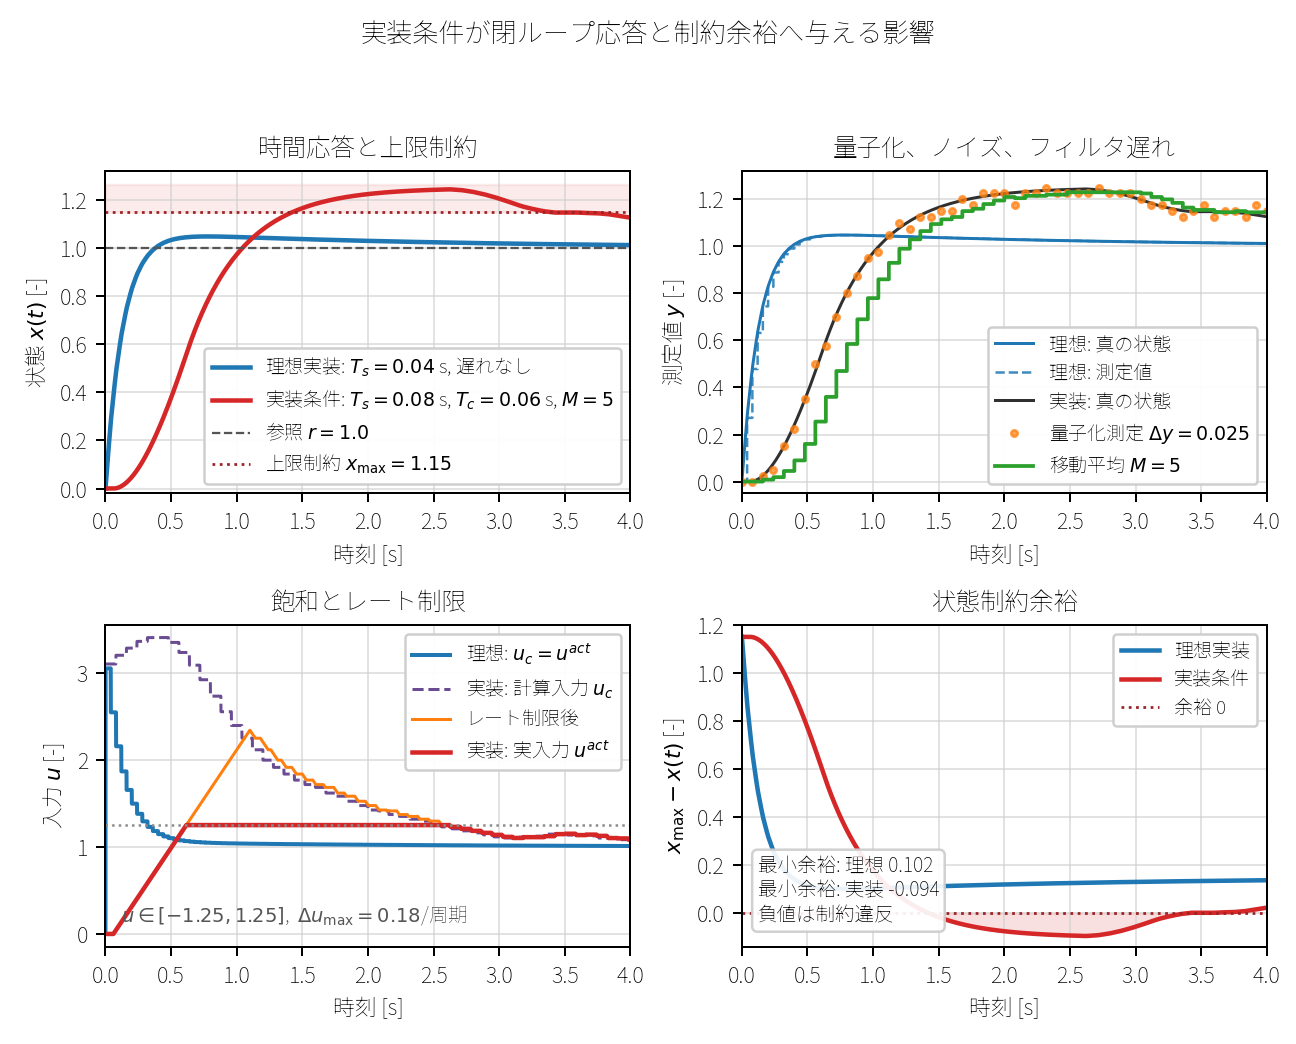
\includegraphics[width=0.96\linewidth,bb=0 0 1296 1044]{figures/implementation_effects_examples.png}
\caption[実装条件による閉ループ応答の比較]{実装条件による閉ループ応答、測定信号、実入力、状態制約余裕の変化。一次遅れ対象を同じ制御器で追従させ、理想的な離散実装と、$T_s=0.08$ [s]、計算遅れ $T_c=0.06$ [s]、量子化幅 $\Delta y=0.025$、移動平均長 $M=5$、入力範囲 $[-1.25,1.25]$、レート制限 $\Delta u_{\max}=0.18$/周期を含む実装を比較している。}
\label{fig:implementation-effects-examples}
\end{figure}

\wfig{implementation-effects-examples} の青線では、測定値が真の状態にほぼ重なり、計算入力と実入力は一本の入力波形として遅れなく対象へ届き、上限制約 $x_{\max}=1.15$ に対して正の余裕が残る。赤線では、量子化と移動平均により制御器が遅れた測定値を見て、計算遅れにより入力がさらに遅れて対象へ届く。入力は上限とレート制限で丸められるため、制御器が求めた $u_c$ と実際の $u^{act}$ が一致しない。この差が予測モデルに入っていないと、時間応答だけでなく制約余裕 $x_{\max}-x(t)$ も過大評価される。したがって、制約付き制御の実装では、サンプリング周期、遅れ、測定フィルタ、量子化幅、入力上下限、入力変化率を、同じシミュレーションまたはログ上で確認する必要がある。次に、測定値と推定値が制御器へ入るまでの実装を式で整理する。

\wfig{implementation-effects-examples} の実装条件では、移動平均長 $M=5$ の低周波遅れは
\begin{equation}
  \frac{(M-1)T_s}{2}
  =\frac{(5-1)\times 0.08}{2}
  =0.16\ \mathrm{s}
\end{equation}
である。ここに計算遅れ $T_c=0.06$ [s] を加えると、制御器から見た代表遅れは $0.16+0.06=0.22$ [s] になる。したがって赤線の制御器は、真の状態より約 $0.22$ [s] 古い情報を基準に $u_c$ を計算している。

入力の下段を見ると、計算された $u_c$ はすぐ大きく変わろうとするが、レート制限後の入力は 1 周期あたり $\Delta u_{\max}=0.18$ までしか変化できず、さらに入力上下限で飽和する。計算遅れを経て対象へ入る $u^{act}$ は、この丸められた入力をさらに遅れて受け取った波形である。したがって状態制約余裕が負になる原因を、測定遅れ、計算遅れ、飽和、レート制限のどれか一つとして切り分けるのは不十分である。測定フィルタと計算遅れは制御判断の時刻を後ろへずらし、飽和とレート制限は予測された入力波形そのものを削るため、制約余裕はこれらを同じログまたは同じシミュレーション内で重ねた閉ループ結果として検証する必要がある。

\subsection{量子化、測定ノイズ、フィルタ、オブザーバ実装}

計算機制御では、物理量そのものではなく、センサ、アナログ回路、A/D 変換器、時刻印、デジタルフィルタ、推定器を通った値を使う。実装上の測定値を
\begin{equation}
  y_k^{m}=Q_{\mathrm{ADC}}\{Cx_k+Du_k^{act}+b_k+v_k\}
\end{equation}
と書く。ここで $u_k^{act}$ は実際に対象へ入った入力、$b_k$ はバイアス、$v_k$ はセンサと回路のランダムノイズ、$Q_{\mathrm{ADC}}$ は A/D 変換による量子化である。制御器が使う予測モデルが $u_k$ ではなく $u_k^{act}$ を必要とする点が重要である。

電圧範囲 $[v_{\min},v_{\max}]$ を $n$ bit の ADC で読むと、代表的な量子化幅は
\begin{equation}
  \Delta_v=\frac{v_{\max}-v_{\min}}{2^n}
\end{equation}
である。端点のコードをどう割り当てるかにより分母を $2^n-1$ とする規約もあるが、設計では使用するデータシートの定義に合わせる。飽和を含めた丸め量子化は
\begin{equation}
  Q_{\mathrm{ADC}}(v)
  =
  \operatorname{clip}_{[v_{\min},v_{\max}]}
  \left(
  v_{\min}
  +\Delta_v
  \operatorname{round}
  \frac{v-v_{\min}}{\Delta_v}
  \right)
\end{equation}
と表せる。入力が飽和しておらず、十分に多くの量子化段をまたいで変化し、量子化誤差が信号と強く相関しないという理想化のもとでは
\begin{equation}
  e_{q,k}=Q_{\mathrm{ADC}}(v_k)-v_k,
  \qquad
  E[e_{q,k}]\simeq0,
  \qquad
  \operatorname{Var}(e_{q,k})\simeq\frac{\Delta_v^2}{12}
\end{equation}
と近似する。したがって、センサ感度が $v=s_y y+v_0$ [V] であれば、物理量 $y$ に換算した量子化ノイズ分散は
\begin{equation}
  R_q=\frac{1}{s_y^2}\frac{\Delta_v^2}{12}
\end{equation}
である。この白色一様ノイズ近似は便利だが、微小振動、低速運動、定常付近の制御では量子化誤差が信号と相関し、階段状の測定値やリミットサイクルとして現れることがある。分解能は「平均すれば常に消える誤差」ではなく、制御対象が見分けられる最小変化量である。

D/A 変換器や PWM 指令にも同じ構造がある。制御器が計算した入力 $u_k^c$ は、出力段で量子化され、さらに物理上限で飽和する。
\begin{equation}
  u_k^{act}
  =
  \operatorname{sat}
  \{Q_{\mathrm{DAC}}(u_k^c)\}
  =
  \min\{u_{\max},\max(u_{\min},Q_{\mathrm{DAC}}(u_k^c))\}
\end{equation}
量子化幅 $\Delta_u$ が大きいと、入力は連続的には変えられず、最小入力変化より小さい補正は対象へ届かない。MPC や制御配分で入力制約を扱うときは、計算上の $u_k^c$ ではなく、実際に実現できる $u_k^{act}$ の範囲、分解能、更新周期を制約に含める。飽和中は線形制御で仮定した入力が実際には入っていないため、積分器、オブザーバ、MPC の状態予測は飽和後の実入力で更新する。

センサノイズには、熱雑音、ショット雑音、増幅器ノイズ、電源リップル、電磁誘導、機械振動、温度ドリフト、オフセット、スケール係数誤差、時刻ジッタ、量子化が含まれる。短時間で平均 0 とみなせる成分は測定ノイズ $v_k$ として
\begin{equation}
  E[v_k]=0,
  \qquad
  E[v_kv_j^\T]=R\delta_{kj}
\end{equation}
と置ける。一方、温度でゆっくり変わるオフセットやセンサのゼロ点ずれは、平均 0 の白色ノイズではなくバイアス状態として
\begin{equation}
  b_{k+1}=b_k+w_{b,k},
  \qquad
  y_k=Cx_k+b_k+v_k+e_{q,k}
\end{equation}
とモデル化する。バイアスを白色ノイズへ押し込むと、フィルタは残差の平均ずれを説明できず、状態推定値でバイアスを代償しようとする。これは制御入力に定常的な偏りを作る原因になる。

ノイズを抑える最も単純なデジタルフィルタは移動平均である。長さ $M$ の移動平均を
\begin{equation}
  \bar{y}_k=\frac{1}{M}\sum_{i=0}^{M-1}y_{k-i}^{m}
\end{equation}
と定義すると、独立な白色ノイズの分散は
\begin{equation}
  \operatorname{Var}(\bar{v}_k)=\frac{1}{M}\operatorname{Var}(v_k)
\end{equation}
へ下がる。$z$ 変換で見ると伝達関数は
\begin{equation}
  H_{\mathrm{MA}}(z)
  =
  \frac{1}{M}\frac{1-z^{-M}}{1-z^{-1}}
\end{equation}
であり、低周波ではおおよそ
\begin{equation}
  H_{\mathrm{MA}}(e^{j\omega T_s})
  \simeq
  e^{-j\omega (M-1)T_s/2}
\end{equation}
の位相遅れを持つ。すなわち、群遅延は約
\begin{equation}
  T_{\mathrm{delay}}\simeq\frac{M-1}{2}T_s
\end{equation}
である。平均を長くすればノイズ分散は下がるが、制御器が古い情報へ反応することになる。

一次の低域フィルタもよく使われる。
\begin{equation}
  \bar{y}_k=(1-\alpha)\bar{y}_{k-1}+\alpha y_k^m,
  \qquad
  0<\alpha\le1
\end{equation}
これは
\begin{equation}
  H_{\mathrm{LP}}(z)
  =
  \frac{\alpha}{1-(1-\alpha)z^{-1}}
\end{equation}
という離散時間伝達関数を持つ。連続時間の一次遅れ時定数 $\tau_f$ を後退 Euler 型に離散化するなら
\begin{equation}
  \alpha=\frac{T_s}{\tau_f+T_s}
\end{equation}
である。低周波での群遅延は近似的に
\begin{equation}
  T_{\mathrm{delay}}
  \simeq
  \frac{1-\alpha}{\alpha}T_s
  =
  \tau_f
\end{equation}
となる。ノイズ抑制と応答性の交換はここに現れる。$\tau_f$ を大きくすると測定値は滑らかになるが、位相余裕が減り、MPC の初期状態も遅れた値から作られる。フィードバックで必要な帯域の近くまでフィルタの遅れが効くなら、ゲインを下げるか、オブザーバのモデル予測を使って測定遅れを補う必要がある。

オブザーバを離散時間で実装するときは、予測と更新を時刻順に分ける。対象と測定を
\begin{align}
  x_{k+1}&=A_dx_k+B_du_k^{act}+w_k,\\
  y_k^{m}&=C_dx_k+D_du_k^{act}+v_k
\end{align}
とし、$u_k^{act}$ は飽和と量子化後に対象へ入った入力であるとする。Luenberger オブザーバの一つの実装形は
\begin{align}
  \hat{x}_{k|k-1}
  &=A_d\hat{x}_{k-1|k-1}+B_du_{k-1}^{act},\\
  \nu_k
  &=y_k^{m}-C_d\hat{x}_{k|k-1}-D_du_{k-1}^{act},\\
  \hat{x}_{k|k}
  &=\hat{x}_{k|k-1}+L\nu_k
\end{align}
である。$\nu_k$ はイノベーション、または予測残差である。誤差 $e_{k|k}=x_k-\hat{x}_{k|k}$ は、ノイズを無視すれば
\begin{equation}
  e_{k|k}=(I-LC_d)A_de_{k-1|k-1}
\end{equation}
に従うので、$L$ は $(I-LC_d)A_d$ の固有値が単位円内に入るように選ぶ。ただし、観測器極を速くしすぎると、測定ノイズと量子化が $L\nu_k$ を通して状態推定値へ強く入る。制御帯域より十分速いが、測定ノイズを過度に増幅しない位置が実装上の選択になる。

Kalman フィルタでは、同じ予測と更新を共分散とともに計算する。
\begin{align}
  \hat{x}_{k|k-1}
  &=A_d\hat{x}_{k-1|k-1}+B_du_{k-1}^{act},\\
  P_{k|k-1}
  &=A_dP_{k-1|k-1}A_d^\T+Q,\\
  S_k
  &=C_dP_{k|k-1}C_d^\T+R,\\
  K_k
  &=P_{k|k-1}C_d^\T S_k^{-1},\\
  \hat{x}_{k|k}
  &=\hat{x}_{k|k-1}+K_k\nu_k
\end{align}
である。共分散更新は丸め誤差に強い Joseph 形
\begin{equation}
  P_{k|k}
  =
  (I-K_kC_d)P_{k|k-1}(I-K_kC_d)^\T
  +K_kRK_k^\T
\end{equation}
を使うと、対称性と半正定性を保ちやすい。$Q$ はモデル化していない外乱やパラメータ誤差を状態へ入れる分散、$R$ はセンサノイズ、回路ノイズ、量子化ノイズを測定単位で足し合わせた分散である。$R$ を小さくしすぎるとフィルタは測定を信じすぎ、量子化段差やスパイクに追従する。$Q$ を小さくしすぎるとモデルを信じすぎ、外乱やバイアス変化に追従できない。

初期化は推定器の一部である。既知の物理状態は $\hat{x}_{0|0}$ へ入れ、不明な状態には大きめの分散を持つ $P_{0|0}$ を置く。すべてを 0 とし、しかも $P_{0|0}=0$ と置くと、フィルタは初期値を完全に正しいと仮定し、測定があっても十分に修正できない。定常運転点が分かるなら
\begin{equation}
  x_0\simeq x_{\mathrm{ss}},
  \qquad
  u_0\simeq u_{\mathrm{ss}}
\end{equation}
を初期値にし、測定出力 $y_0^m$ から観測可能な成分だけを最小二乗で合わせる。測定が飽和している、範囲外でクリップされている、または時刻印が欠けている場合には、そのサンプルを通常の $R$ で更新してはならない。更新を飛ばす、該当成分の $R$ を大きくする、または測定飽和を不等式情報として扱う。

実装後の健全性確認では、共分散と残差を見る。共分散は常に
\begin{equation}
  P_{k|k}=P_{k|k}^\T,
  \qquad
  P_{k|k}\ge0
\end{equation}
でなければならない。数値丸めで非対称になった場合には $(P+P^\T)/2$ に戻すが、負の固有値が大きく出るなら $Q$、$R$、離散化、時刻順序、単位換算の誤りを疑う。イノベーション共分散 $S_k$ は正定でなければならず、正規化イノベーション
\begin{equation}
  \epsilon_k=\nu_k^\T S_k^{-1}\nu_k
\end{equation}
は測定次元と同程度の大きさで推移するのが一つの目安である。$\epsilon_k$ が継続して大きいなら、モデル誤差、バイアス、外れ値、過小な $R$ が疑われる。継続して小さすぎるなら、$R$ を過大に置いて測定を捨てすぎている可能性がある。

小さな数値例で量子化とフィルタ遅れを見積もる。$0$--$100$ [$^\circ$C] の温度を $0$--$5$ [V] に変換するセンサを、12 bit ADC で読む。分解能は
\begin{align}
  \Delta_v&=\frac{5}{4096}\simeq1.22\times10^{-3}\ \mathrm{V},\\
  \Delta_T&=\frac{100}{4096}\simeq2.44\times10^{-2}\ {^\circ\mathrm{C}}
\end{align}
であり、量子化を一様ノイズとみなすと
\begin{equation}
  \sigma_q=\frac{\Delta_T}{\sqrt{12}}
  \simeq7.0\times10^{-3}\ {^\circ\mathrm{C}}
\end{equation}
である。センサ自身の標準偏差が $0.05$ [$^\circ$C] なら、Kalman フィルタの測定分散として
\begin{equation}
  R\simeq(0.05)^2+(0.0070)^2
  \simeq2.55\times10^{-3}\ ({^\circ\mathrm{C}})^2
\end{equation}
を初期値にできる。サンプリング周期 $T_s=0.05$ [s] で $M=8$ の移動平均を入れると、白色ノイズ分散は約 $1/8$ になるが、遅れは
\begin{equation}
  T_{\mathrm{delay}}\simeq\frac{7}{2}T_s=0.175\ \mathrm{s}
\end{equation}
である。熱時定数が 5 [s] の温度制御ならこの遅れは小さいことが多い。一方、時定数が 0.3 [s] の速度制御で同じ遅れを入れると、位相遅れは閉ループ帯域の近くで支配的になり得る。ノイズを下げる設計は、必ず応答遅れと制約余裕の消費として評価する。

\subsection{アクチュエータ非線形性と制約実装}

アクチュエータの非線形性は、制御器の外側で最後に作用する誤差ではなく、対象へ入る入力写像そのものである。計算機が出す指令を $u_{c,k}$、対象へ実際に入る入力を $u_k$ と書くと、離散時間の実装モデルは
\begin{align}
  u_k&=\psi(u_{c,k},u_{k-1},\eta_k),\\
  x_{k+1}&=f_d(x_k,u_k,w_k)
\end{align}
と表すのが基本である。$\psi$ はアクチュエータ、ドライバ、機械伝達部、保護回路をまとめた入力写像であり、$\eta_k$ は摩擦状態、すきまの接触向き、温度などの内部状態を表す。線形制御の設計式では $u_k=u_{c,k}$ を仮定するが、実機では $\psi$ が飽和、レート制限、デッドゾーン、バックラッシュ、ヒステリシスを含む。この差を無視すると、状態予測、オブザーバ、積分器が、対象へ入っていない入力を入ったものとして扱う。

上下限飽和は最も直接的な非線形性である。各成分ごとに
\begin{equation}
  u_k=\operatorname{sat}(u_{c,k})
  =\min\{u_{max},\max(u_{min},u_{c,k})\}
\end{equation}
と書ける。ここで $u_{min}$、$u_{max}$ は物理的に実現可能な入力下限と上限であり、単位は入力 $u$ と同じである。飽和中は $\partial u_k/\partial u_{c,k}=0$ とみなせる領域が生じるため、入力を増やす指令は対象の加速度、流量、熱量を増やさない。MPC ではこの制限を
\begin{equation}
  u_{min}\le u_{i|k}\le u_{max}
\end{equation}
というハード制約として予測問題に入れる。ソルバの外側で飽和させるだけだと、最適化は実現不能な入力に基づいて将来状態を予測し、実際の閉ループは予測より遅れて制約境界へ近づく。

レート制限は、入力値そのものではなく一サンプルあたりの入力変化を制限する。サンプリング周期を $T_s$ [s]、連続時間の最大変化率を $\dot{u}_{max}$ [入力単位/s] とすれば、離散時間で許される変化幅は
\begin{equation}
  \Delta u_{max}=T_s\dot{u}_{max}
\end{equation}
である。計算指令 $u_{c,k}$ を受けた後の実入力は
\begin{align}
  u_k
  &=u_{k-1}
  +\operatorname{sat}_{[-\Delta u_{max},\,\Delta u_{max}]}
    (u_{c,k}-u_{k-1})\\
  &=\min\{u_{k-1}+\Delta u_{max},
      \max(u_{k-1}-\Delta u_{max},u_{c,k})\}
\end{align}
で表せる。MPC の予測では、過去に実際へ出た $u_{k-1}$ を初期条件として
\begin{equation}
  -\Delta u_{max}
  \le u_{i|k}-u_{i-1|k}
  \le \Delta u_{max}
  \qquad (i=0,\ldots,N_p-1)
\end{equation}
を課す。ただし $u_{-1|k}=u_{k-1}$ である。レート制限を入れると、入力が上限に達していなくても、急な回避や急な追従に必要な入力列が作れない場合がある。したがって安全制約の余裕は、入力振幅だけでなく入力速度の制約からも決まる。

デッドゾーンは、小さい指令が機械摩擦、弁の重なり、モータドライバの不感帯などに吸収され、対象へ伝わらない非線形性である。幅 $d>0$ の対称デッドゾーンは
\begin{equation}
  u_k=\operatorname{dz}(u_{c,k})=
  \begin{cases}
    0, & \abs{u_{c,k}}\le d,\\
    u_{c,k}-d, & u_{c,k}>d,\\
    u_{c,k}+d, & u_{c,k}<-d
  \end{cases}
\end{equation}
と書ける。デッドゾーンを持つ対象では、小さな偏差に対して制御器が指令を出していても実入力は 0 になり、定常偏差または微小振動が残る。補償として、指令にオフセットを加える逆デッドゾーンを使うことはあるが、符号反転付近では不連続な切替が入り、ノイズにより入力符号が頻繁に反転しやすい。MPC では、デッドゾーンを非線形予測モデルに入れるか、少なくとも小入力領域では期待した入力効果が得られないものとして制約余裕と重みを設計する。

バックラッシュは、歯車、リンク、ねじ機構などのすきまにより、入力側の変位がすぐには出力側へ伝わらない現象である。入力側変位を $q_k$、出力側変位を $y_k$、すきま幅を $2b$ とすると、簡単な離散表現は
\begin{equation}
  y_k=
  \begin{cases}
    q_k-b, & q_k-y_{k-1}>b,\\
    q_k+b, & q_k-y_{k-1}<-b,\\
    y_{k-1}, & \abs{q_k-y_{k-1}}\le b
  \end{cases}
\end{equation}
である。中央の領域では入力側だけが動き、出力側は前の位置に保持される。ヒステリシスは、同じ現在入力でも、過去に増加側から来たか減少側から来たかで出力が変わる履歴依存性である。バックラッシュもヒステリシスも、単なる静的関数 $u=\phi(u_c)$ ではなく、内部状態を持つ写像として扱う必要がある。予測モデルへ入れるなら、接触向きや履歴変数を状態に加え、切替境界での不連続性または不滑らか性を認識して NMPC やシミュレーション検証を行う。

飽和と積分器は、特に windup を通じて結びつく。PI 制御器を
\begin{align}
  z_{I,k+1}&=z_{I,k}+T_se_k,\\
  u_{c,k}&=K_pe_k+K_iz_{I,k}
\end{align}
と実装し、実入力が $u_k=\operatorname{sat}(u_{c,k})$ で決まるとする。飽和中に誤差 $e_k$ が同じ符号で残ると、積分状態 $z_{I,k}$ は増え続けるが、実入力 $u_k$ はこれ以上増えない。制約から離れた後も大きく蓄積した積分状態が残り、応答の戻り過ぎや長い整定時間を生む。代表的な anti-windup の一つは逆計算であり、
\begin{equation}
  z_{I,k+1}
  =z_{I,k}+T_se_k
  +K_{aw}(u_k-u_{c,k})
\end{equation}
と更新する。$u_k-u_{c,k}$ は、計算指令と実入力の差である。飽和で $u_c$ が大き過ぎるとこの項が積分状態を戻す向きに働く。積分器だけでなく、外乱推定器やオブザーバに入力を入れる場合も、更新に使うべき値は $u_{c,k}$ ではなく飽和、レート制限、デッドゾーンを通過した後の $u_k$ である。

MPC では、入力非線形性を制約として扱えるものと、モデルとして扱うべきものを分ける。上下限とレート制限は線形不等式であり、リフトアップした入力列 $U$ に対して
\begin{equation}
  \begin{bmatrix}
    I\\-I\\D\\-D
  \end{bmatrix}U
  \le
  \begin{bmatrix}
    \mathbf{1}u_{max}\\-\mathbf{1}u_{min}\\
    \mathbf{1}\Delta u_{max}+d_0\\
    \mathbf{1}\Delta u_{max}-d_0
  \end{bmatrix}
\end{equation}
の形に積み上げられる。$D$ は隣り合う入力差を作る行列であり、$d_0$ は初期差分に現れる既知の $u_{k-1}$ を右辺へ移した項である。一方、デッドゾーン、バックラッシュ、ヒステリシスは、一般には非凸または履歴依存の非線形性である。線形 MPC にそのまま入れる代わりに、運転範囲を限定して余裕を縮小する、下位ループで補償して上位 MPC へ有効な制約を返す、または NMPC の状態として明示する、という選択をする。

安全上の意味は、入力指令が安全制約を満たすことと、実入力が安全制約を守れることを区別する点にある。非常停止で入力を 0 にしても、レート制限やバックラッシュにより力や流量がすぐ 0 へ変わらない場合がある。反対に、上位制御器が回避入力を要求しても、飽和、デッドゾーン、すきま詰めの時間により必要な入力が遅れて届く場合がある。したがって安全集合 $\mathcal{X}_{\mathrm{safe}}$ は、名目モデルだけでなく、入力振幅、入力速度、非線形伝達、最悪遅れを含む到達可能集合で確認する。ソルバが成功しても、実入力が予測入力と異なるなら、その成功は安全保証にならない。

一次遅れ温度系の簡単な数値例を考える。
\begin{equation}
  x_{k+1}=0.9x_k+0.4u_k,
  \qquad
  \abs{u_k}\le1,
  \qquad
  \abs{u_k-u_{k-1}}\le0.2
\end{equation}
現在 $x_k=2$、前回入力 $u_{k-1}=0$ とし、状態を早く下げるために制御器が $u_{c,k}=-1$ を要求したとする。振幅制限だけを考えれば $u_k=-1$ を許せるが、レート制限後の実入力は
\begin{equation}
  u_k=\max(-0.2,\min(0.2,-1))=-0.2
\end{equation}
であり、次状態は
\begin{equation}
  x_{k+1}=0.9\cdot2+0.4(-0.2)=1.72
\end{equation}
にしか下がらない。予測で $u=-1$ を使えば $x_{k+1}=1.4$ と見積もるため、安全上限が $x\le1.6$ の近くにある場合、名目予測は安全余裕を過大評価する。同じ制約を MPC に入れると、時刻 $k$ では $u_{0|k}\ge-0.2$、次時刻でも $u_{1|k}\ge-0.4$ という列制約が現れ、状態制約を満たせないなら早い時刻から減速する、参照を緩める、または安全側制御へ切り替える判断が可能になる。

\subsection{安全制約、フェイルセーフ、監視ロジック}

安全制約は、性能を少し悪くしても越えてよい制約ではなく、制御器の有効範囲そのものを定める制約である。状態の安全集合を
\begin{equation}
  \mathcal{X}_{\mathrm{safe}}
  =
  \{x\mid h_j(x)\le0,\ j=1,\ldots,n_h\}
\end{equation}
と書く。$h_j(x)$ は温度上限、位置範囲、圧力上限、速度上限のような物理量を表す関数であり、単位とセンサ換算を明示しておく必要がある。MPC の経路制約としては
\begin{equation}
  h_j(x_{i|k})\le0
  \qquad (i=1,\ldots,N)
\end{equation}
を置けるが、これだけでは安全設計は閉じない。予測外乱、推定誤差、遅れ、入力制限、ソルバ失敗時の入力を含めても、実際の状態が集合内に残ることを別に確認しなければならない。

ハード制約とソフト制約の区別はここで本質的になる。ハード制約は、最適化問題の実行可能解として必ず満たす制約である。ソフト制約は、スラック変数で違反を数値的に罰する制約であり、たとえば
\begin{align}
  h_j(x_{i|k})&\le s_{j,i},\\
  s_{j,i}&\ge0,\\
  J&\leftarrow J+\rho_j s_{j,i}+\frac{1}{2}w_j s_{j,i}^{2}
\end{align}
と書ける。ソフト制約は、参照追従、快適性、経済性、望ましい運転範囲のように、違反量を記録して小さく抑えれば制御を継続できる条件に使う。一方、衝突、過熱、過圧、機械ストッパ、電流の絶対上限のような不可侵条件をソフト化すると、最適解が「少し危険側へ出る」ことを許してしまう。したがって、安全制約は原則としてハード制約に残し、どうしても緩和が必要な場合でも、ハードな外側限界とソフトな内側警告限界を分ける。
\begin{align}
  h_j^{\mathrm{hard}}(x_{i|k})&\le0,\\
  h_j^{\mathrm{warn}}(x_{i|k})&\le s_{j,i}
\end{align}
この二重化により、最適化は警告領域への侵入を避けようとするが、物理的な安全限界は実行可能性の条件として残る。

安全集合は、単に望ましい範囲を描いた集合では不十分である。離散時間モデル
\begin{equation}
  x_{k+1}=f_d(x_k,u_k,w_k),
  \qquad
  w_k\in\mathcal{W}
\end{equation}
に対し、集合 $\mathcal{C}\subseteq\mathcal{X}_{\mathrm{safe}}$ が制御不変集合であるとは、任意の $x\in\mathcal{C}$ に対して、許された入力 $u\in\mathcal{U}$ が存在し、すべての外乱 $w\in\mathcal{W}$ について
\begin{equation}
  f_d(x,u,w)\in\mathcal{C}
\end{equation}
が成り立つことである。安全限界の内側にいても、そこから一サンプル後に避ける入力が存在しないなら、その状態は安全に回復可能な状態ではない。MPC の終端集合やフェイルセーフ制御則は、できれば $\mathcal{X}_{\mathrm{safe}}$ 全体ではなく、その内側の制御不変集合 $\mathcal{C}$ へ接続するように設計する。

外乱と推定誤差を明示すると、名目予測と実状態はずれる。名目状態を $\bar{x}_{i|k}$、誤差を $e_{i|k}=x_{k+i}-\bar{x}_{i|k}$ とし、誤差集合を
\begin{equation}
  e_{i|k}\in\mathcal{E}_i
\end{equation}
と見積もる。真の状態を安全集合に残すには、名目状態を内側へ縮めた集合に入れる。
\begin{equation}
  \bar{x}_{i|k}
  \in
  \mathcal{X}_{\mathrm{safe}}\ominus\mathcal{E}_i
\end{equation}
半空間制約 $Hx\le h$ では、この縮小は各行ごとに
\begin{equation}
  H_j\bar{x}_{i|k}
  \le
  h_j-\max_{e\in\mathcal{E}_i}H_je
\end{equation}
と書ける。右辺の差し引き量が安全余裕である。オブザーバの推定誤差共分散 $P_{k|k}$ を使う場合には、確率水準 $\alpha$ に対して
\begin{equation}
  \mathcal{E}_k(\alpha)
  =
  \{e\mid e^\T P_{k|k}^{-1}e\le\alpha\}
\end{equation}
のような楕円体を誤差集合の近似に使う。ただし、これはフィルタのモデル、ノイズ仮定、外れ値処理が妥当な場合の近似であり、センサ故障やバイアスの急変を含む保証ではない。残差が異常なときは、$P$ で作った余裕をそのまま信用せず、測定更新を弱める、誤差集合を広げる、または安全側モードへ移る。

異常検知の基本量は、予測出力と測定出力の残差である。オブザーバまたは Kalman フィルタの予測を使い
\begin{align}
  \hat{y}_{k|k-1}
  &=C_d\hat{x}_{k|k-1}+D_du_{k-1}^{act},\\
  r_k
  &=y_k^m-\hat{y}_{k|k-1}
\end{align}
と定義する。正常時の残差共分散を $S_k$ と見積もれるなら、正規化残差
\begin{equation}
  \epsilon_k=r_k^\T S_k^{-1}r_k
\end{equation}
を監視する。測定次元を $m$ とし、残差が平均 0 の Gaussian 近似に従うなら、$\epsilon_k$ はおおよそ自由度 $m$ の $\chi^2$ 分布に従う。しきい値 $\gamma$ は
\begin{equation}
  \Pr\{\chi_m^2>\gamma\}=p_{\mathrm{FA}}
\end{equation}
のように、許容する誤警報確率 $p_{\mathrm{FA}}$ から初期値を決められる。ただし、実データではノイズが完全な白色 Gaussian でないことが多いため、ログで正常時分布を確認し、温度、運転点、量子化、フィルタ遅れによる偏りを含めて調整する。

単一のしきい値だけでモードを切り替えると、ノイズにより正常と異常を頻繁に往復する。これを避けるため、しきい値にヒステリシスと継続時間を入れる。たとえば異常判定用しきい値を $\gamma_{\mathrm{on}}$、復帰用しきい値を $\gamma_{\mathrm{off}}$ とし、
\begin{equation}
  \gamma_{\mathrm{off}}<\gamma_{\mathrm{on}}
\end{equation}
を満たすように選ぶ。連続超過回数 $n_k^{+}$ と連続正常回数 $n_k^{-}$ を
\begin{align}
  n_k^{+}
  &=
  \begin{cases}
    n_{k-1}^{+}+1, & \epsilon_k>\gamma_{\mathrm{on}},\\
    0, & \epsilon_k\le\gamma_{\mathrm{on}},
  \end{cases}\\
  n_k^{-}
  &=
  \begin{cases}
    n_{k-1}^{-}+1, & \epsilon_k<\gamma_{\mathrm{off}},\\
    0, & \epsilon_k\ge\gamma_{\mathrm{off}}
  \end{cases}
\end{align}
と更新し、$n_k^{+}\ge N_{\mathrm{on}}$ で異常モードへ入り、$n_k^{-}\ge N_{\mathrm{off}}$ で復帰を許す。この設計では、検出遅れはおよそ $N_{\mathrm{on}}T_s$ だけ増える。安全余裕はこの遅れの間にも制約へ到達しないように設計する。

監視ロジックは、残差だけでなく、計算時間、ソルバ終了状態、制約違反、通信、センサ範囲、アクチュエータ応答を同時に見る。時刻 $k$ で制御入力を採用できる条件を
\begin{align}
  q_k=1
  \Longleftrightarrow
  &\ T_{\mathrm{solve},k}\le T_{\max},\\
  &\ \mathrm{status}_k=\mathrm{success},\\
  &\ \epsilon_k\le\gamma_{\mathrm{on}},\\
  &\ \hat{x}_{k|k}\in\mathcal{X}_{\mathrm{safe}}\ominus\mathcal{E}_0,\\
  &\ u_k^{act}\in\mathcal{U},\quad \Delta u_k^{act}\in\Delta\mathcal{U}
\end{align}
のような論理式で定める。実装ではこの条件を制御計算とは別の監視タスクにも置き、監視タイマにより時刻印が進んでいるか、入力が更新されているか、前回の有効解が古くなりすぎていないかを検査する。最適化問題が成功しても、計算締切を過ぎた入力は現在状態に対する入力ではない。逆に、最適化が失敗しても前回入力を保持すれば安全とは限らない。保持入力で安全集合に残れる時間も設計量である。

フェイルセーフ入力は、異常を検出してから考えるのではなく、通常時から制御器の一部として定義する。代表的なモードを
\begin{equation}
  \mathcal{M}_k\in
  \{\mathrm{normal},\mathrm{degraded},\mathrm{safe}\}
\end{equation}
とし、入力選択を
\begin{equation}
  u_k=
  \begin{cases}
    u_k^{\mathrm{MPC}}, & \mathcal{M}_k=\mathrm{normal},\ q_k=1,\\
    u_k^{\mathrm{deg}}(\hat{x}_k,u_{k-1}^{act}), & \mathcal{M}_k=\mathrm{degraded},\\
    u_k^{\mathrm{safe}}(\hat{x}_k,u_{k-1}^{act}), & \mathcal{M}_k=\mathrm{safe}
  \end{cases}
\end{equation}
と明示する。劣化運転では、参照を安全側へ近づけ、重みを保守的にし、入力変化率と運転範囲を狭める。たとえば
\begin{equation}
  r_{i|k}^{\mathrm{deg}}
  =
  (1-\beta_k)r_{i|k}
  +\beta_k r_{\mathrm{safe}},
  \qquad
  0\le\beta_k\le1
\end{equation}
とすれば、$\beta_k$ を大きくするほど参照は安全な定常点へ近づく。安全モードでは、低ゲイン局所制御、制限付き入力保持、制動入力、入力遮断などを対象の物理に合わせて選ぶ。重要なのは、$u_k^{\mathrm{safe}}$ 自身が入力上下限、レート制限、むだ時間を含めて実現可能であり、集合 $\mathcal{C}$ へ入る、または少なくとも $\mathcal{X}_{\mathrm{safe}}$ の外へ出るまでの時間を最大化することである。

MPC と監視器の相互作用では、どの情報を信じて制約を課すかが問題になる。MPC はふつう推定状態 $\hat{x}_{k|k}$ から予測を始めるため、制約は
\begin{equation}
  \hat{x}_{i|k}\in\mathcal{X}_{\mathrm{safe}}\ominus\mathcal{E}_{i|k}
\end{equation}
の形で推定誤差を含める。残差が大きいときに $\hat{x}_{k|k}$ をそのまま使うと、誤った状態から正確な最適化問題を解くことになる。したがって、異常検知が働いたら、測定更新を飛ばすだけでなく、MPC の初期誤差集合を広げ、制約をさらに締め、参照を緩める。必要なら、MPC の出力を採用せず、直前に検証済みの安全側入力へ切り替える。

安全設計の最小構成は、主制御器、状態推定器、監視器、フェイルセーフ制御器を別々の役割として持つことである。主制御器は性能と制約を同時に扱い、推定器は状態と残差を与え、監視器は「その制御入力を採用してよいか」を判定し、フェイルセーフ制御器は主制御器が使えないときの入力を与える。数式で書けば、閉ループは
\begin{align}
  \hat{x}_{k|k},r_k,S_k
  &\leftarrow \mathrm{observer}(y_k^m,u_{k-1}^{act}),\\
  u_k^{\mathrm{MPC}}
  &\leftarrow \mathrm{optimizer}(\hat{x}_{k|k},\mathcal{X}_{\mathrm{safe}}\ominus\mathcal{E}),\\
  \mathcal{M}_k
  &\leftarrow \mathrm{monitor}(r_k,S_k,T_{\mathrm{solve},k},\mathrm{status}_k),\\
  u_k
  &\leftarrow \mathrm{select}(u_k^{\mathrm{MPC}},u_k^{\mathrm{deg}},u_k^{\mathrm{safe}},\mathcal{M}_k)
\end{align}
と整理できる。この分解により、MPC の最適性、オブザーバの統計的整合性、監視器の検出遅れ、フェイルセーフ入力の到達可能性を個別に検証できる。安全制約は、最適化問題の一行としてだけでなく、推定誤差、実入力、監視遅れ、異常時モードまで含む閉ループの性質として扱う必要がある。

\subsection{階層的な実時間制御}

複雑な機械の制御器は、時間スケールに基づいて階層化されることが多い。遅い層では目標軌道や制約付き最適化を扱い、中間層では状態フィードバックや配分を行い、速い層では電流、速度、力などの局所ループを閉じる。

たとえば上位の MPC が一般化力 $w_k$ を決め、中位の配分がアクチュエータ入力 $u_k$ へ変換し、下位の PI ループが実際のモータ速度を追従させる。推定器は各層へ状態を供給し、ログと診断はモデル誤差の検出に用いられる。全体は
\begin{equation}
  \text{推定}\rightarrow \text{予測}\rightarrow \text{配分}\rightarrow \text{局所制御}\rightarrow \text{対象}
\end{equation}
という循環になる。

階層化しても、各層は独立ではない。上位層の目標が下位層の帯域や入力制限を超える場合、飽和または追従遅れが生じる。したがって、上位層の制約には下位層の限界を含め、下位層の状態を上位層へ戻す構成が必要である。

ここから後の項目は、新しい話題を横に並べる部分ではなく、\wfig{mpc-architecture} の最適化器から対象へ向かう一本の経路を分解する部分である。制約条件は KKT 条件で診断し、線形 MPC は QP の行列として実装し、非線形モデルでは直接法と RTI により同じ経路を近似する。さらに、最適化器が求めた一般化力は制御配分で実アクチュエータへ移され、\wfig{implementation-effects-examples} で見た実入力、遅れ、量子化、制約余裕に戻って検証される。各小節では、直前の式が前半の図のどの信号、制約、余裕を固定しているかを、式変形、図中の信号対応、実装上の余裕評価として本文中で確認していく。
